\section{Nichtdeterministische Kellerautomat}

NEA:$A=(Q,\Sigma,\Gamma,\delta,q_{0},k_{0},F)$ (pda)\\
$Q$ Zustandsmenge, nichtleer \& endlich\\
$\Sigma$Eingabealphabet $(Q\cap\Sigma=\emptyset)$\\
$\Gamma$Kelleralphabet $(Q\cap\Gamma=\emptyset)$\\
$\delta$Transitionsfunktion, Abbildung von $Q\times(\Sigma\cup\epsilon)\times\Gamma$(Zustand,
Eingabewort, gelesen vom Stapel), im Keller muss immer min. ein Symbol
vorhanden sein; $\delta(q_{i},a,k)\rightarrow\delta(Zustand,gelesenesZeichen,gelesenesKellerzeichen)$
\\
$q_{0}$Anfangszustand, $q_{0}\in Q$\\
$k_{0}$Anfangskellersymbol, $k_{0}\in\Gamma$\\
$F$ Menge der Endzustände, $E\subseteq Q$\\
Ist das Bild von $\delta$ niemals die leere Menge, nennt man A einen
\emph{vollständigen nichtdeterministischen Automaten}. Vom Keller
gelesene Symbole werderden gelöscht und müssen sofern es nocht benötigt
wird wieder zurück in den Keller geschrieben werden. Es gibt nur Möglichkeiten,
entweder der Automat hat im Endzustand einen leeren Keller oder beinhaltet
die Markierung für das Ende ($k_{0})$.


\subsection{Konfiguration}

$A=(Q,\Sigma,\Gamma,\delta,q_{0},k_{0},F)$ sei ein NEA
\begin{enumerate}
\item Jedes Tripel $(q,w,\gamma)\in Q\times\Sigma^{*}\times\Gamma^{*}$heißt
\emph{Konfiguration} des Kellerautomaten A
\item Die Konfiguration $(q_{0},w,k_{0})$ heißt \emph{Anfangskonfiguration}
des Automaten bei Eingabe des Wortes $w$
\item Der Übergang $\vdash$von einer Konfiguration zur nächsten ist für
alle $q_{i}\in Q$, $a_{i}\in\Sigma\cup\{\epsilon\}$ (Zeichen in
w gehört zum Eingabealphabet oder ist $\epsilon$), $k\in\Gamma^{*}$(k
gehört zum Kelleralphabet inkl.$\epsilon$), $w\in\Sigma^{*}$(das
Wort ist im Eingabealphabet enthalten inkl. leer) und für alle Wörter
$\gamma\in\Gamma^{*}$(Jedes Gamma ist enthalten im Kelleralphabet
inkl. $\epsilon$) definiert durch:\\
$(q_{i},aw,k\gamma)\vdash(q_{j},w,\gamma_{1}\gamma$) (der Übergang
ist dann möglich wenn $(q_{i,}\gamma_{i})$ in der Transitionsfunktion
$\delta(q_{i},a,k)$ enthalten sind\\
\emph{a} wird gelesen und \emph{k} wird durch $\gamma_{1}$ersetzt,
der Zustand $q_{i}$wechselt in den Zustand $q_{j}$. Die Konfiguration
$(q_{j},w,\gamma_{1}\gamma)$wird \emph{Folgekonfiguration} von $(q_{i},aw,k\gamma)$genannt.
\item Wenn eine Konfiguration $(q_{i},w_{i},\gamma_{i})$ nach \emph{n}
$(n\ge0)$ Folgekonfigurationen die Konfiguration $(q_{j},w_{j},\gamma_{j})$
erreicht, dann schreibe ich $(q_{i},w_{i},\gamma_{i})\vdash^{*}(q_{j},w_{j},\gamma_{j})$
\end{enumerate}

\section*{Beispiel:}

Sprache:$L=\{a^{n}b^{n}|n\in\mathbb{N})\subseteq\{a,b\}^{*}$\\
Konstruktionsidee für $A=(Q,\Sigma,\Gamma,\delta,q_{0},k_{0},F)$:

$Q=\{q_{0},q_{1},q_{2}\}$- Mögliche Zustände des Automaten

$\Sigma=\{a,b\}$- \emph{Eingabealphabet}

$\Gamma=\{k_{0},a\}$- \emph{Kelleralphabet}

$F=\{q_{2}\}$- Endzustände

$\delta$wird definiert für die folgenden Argumente:

\begin{eqnarray}
\delta(q_{0},a,k_{0}) & = & \{(q_{0},ak_{0})\}\\
\delta(q_{0},a,a) & = & \{(q_{0},aa)\}\}\\
\delta(q_{0},b,a) & = & \{(q_{1},\epsilon)\}\\
\delta(q_{1},b,a) & = & \{(q_{1},\epsilon)\}\\
\delta(q_{1},\epsilon,k_{\text{0}}) & = & \{(q_{2},k_{0})\}\\
\text{für alle anderen Argumente} &  & (q,x,z)\in Qx(\Sigma\bigcup\{\epsilon\}x\Gamma\text{ist}\delta(q,x,z)=\emptyset
\end{eqnarray}


Konfigurationsfolge$w=aabb$

$(q_{0},aabb,k_{0})\vdash(q_{0},abb,ak_{0})\vdash(q_{0},bb,aak_{0})\vdash(q_{0},b,ak_{\text{0}})\vdash(q_{1},\epsilon,k_{0})\vdash(q_{2},\epsilon,k_{0})$

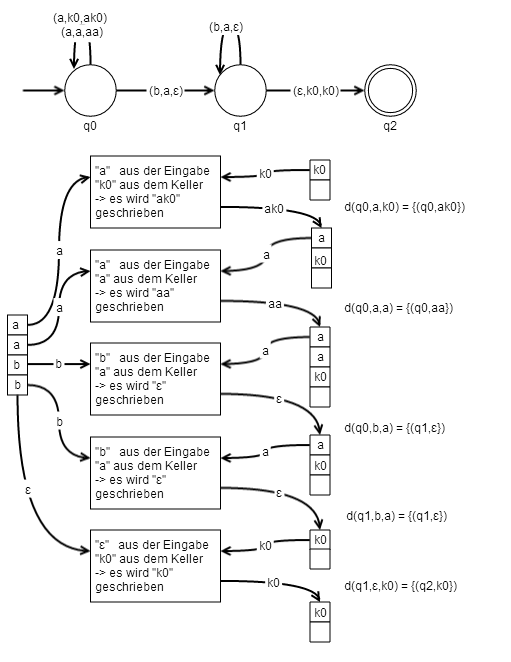
\includegraphics{kellerautomat}


\subsection{Akzeptierte Sprachen eines NEA}

Wesentlich für die Akzeptanz einers Wortes ist:
\begin{enumerate}
\item \emph{Akzeptieren mit Entzuständen}

\begin{enumerate}
\item Das Wort muss komplett gelesen werden
\item Nachdem das Wort ganz gelesen wurde, muss ein Endzustand erreicht
werden (es können vor/nach dem erreichen des Endzustands noch weitere
Zustände durchlaufen werden)
\item Der Automat muss nicht anhalten
\item Der Keller muss nicht leer sein (Reste von ``Nebenberechnungen''
können noch enthalten sein)
\end{enumerate}
\item \emph{Akzeptieren mit leerem Keller}

\begin{enumerate}
\item Das Wort muss ganz gelesen werden
\item Nachdem das Wort ganz gelesen wurde, muss auch der Keller ganz geleert
sein oder geleert werden
\item Der Zustand, in dem sich der Automat befindet, ist beliebig (er muss
kein Endzustand sein)
\item Der Automat hält weil der Keller leer ist. Mit leerem Keller kann
der Automat nicht arbeiten (d.h. auch kein Marker $k_{0}$darf mehr
enthalten sein). Die Endzustandsmenge ist hierbei willkürlich!
\end{enumerate}
\end{enumerate}

\subsection{Kontextfreie Sprachen \& nichtdeterministische Kellerautomaten}

Jede kontextfreie Sprache wird von einem Kellerautomaten akzeptiert.


\subsection{Abschlusseingenschaften kontextfreie Sprachen}

Der Durchschnitt einer kontextfreier Sprachen ist im Allgemeinen nicht
kontextfrei.

Das Komplement einer kontextfreien Sprachen ist ebenfalls im Allgemeinen
keine kontextfreie Sprache.

Der Durchschnitt einer kontextfreien Sprache mit einer regulären Sprache
ist eine kontextfreien Sprachen.


\section{Deterministische Kellerautomaten}

Ein Kellerautomat $A=(Q,\Sigma,\Gamma,\delta,q_{0},k_{0},F)$ ist
ein deterministischer Kellerautomat (dpda), wenn die Transitionsfunktion
$\delta$die folgenden Eigenschaften hat:

Für alle $(q,x,k)\in Q\times(\Sigma\cup\{\epsilon\})\times\Gamma$ist
\begin{enumerate}
\item $|\delta(q,x,k)|\leq1$und
\item falls $\delta(q,\epsilon,k)\neq\emptyset$ist, dann ist für alle $a\in\Sigma$:
$\delta(q,a,k)=\emptyset$
\end{enumerate}

\subsection{Deterministische kontextfreie Sprache}

$A=(Q,\Sigma,\Gamma,\delta,q_{0},k_{0},F)$ sei ein deterministischer Kellerautomat. Die Menge $L(A)=\{w|(q_{0},w,k_{0})\vdash^{*}(q,\epsilon,\gamma),q\in F,\gamma\in\Gamma^{*}\}\subseteq\Sigma^{*}$ist
die von dem deterministischen Kellerautomaten A akzeptierte Sprache.
Sie heißt \emph{deterministische kontextfreie Sprache}.


\section*{Beispiel:}

\emph{dpda} für $L=\{a^{n}b^{n}|n\in\mathbb{N}\}\subseteq\{a,b\}^{*}$

Der Automat $A=(Q,\Sigma,\Gamma,\delta,q_{\text{0}},k_{0},F)$:

$Q=\{q_{0},q_{1},q_{2}\}$

\emph{$\Gamma=\{k_{0},a\}$}

$F=\{q_{2}\}$

$\delta$ definiert durch:

$\delta(q_{0},a,k_{0}\}=(q_{0},k_{0})$ $\delta(q_{0},a,a)=(q_{0},aa)$
$\delta(q_{0},b,a)=(q_{1},\epsilon)$ \newline
$\delta(q_{1},b,a)=(q_{1},\epsilon)$ $\delta(q_{1},b,k_{0})=(q_{2},k_{0})$

ist ein deterministische Kellerautomat